\documentclass[border=10pt]{standalone}
\usepackage[T1]{fontenc}\usepackage[utf8]{inputenc}\usepackage{lmodern}
\usepackage{tikz}\usetikzlibrary{arrows.meta,positioning,calc}
\begin{document}
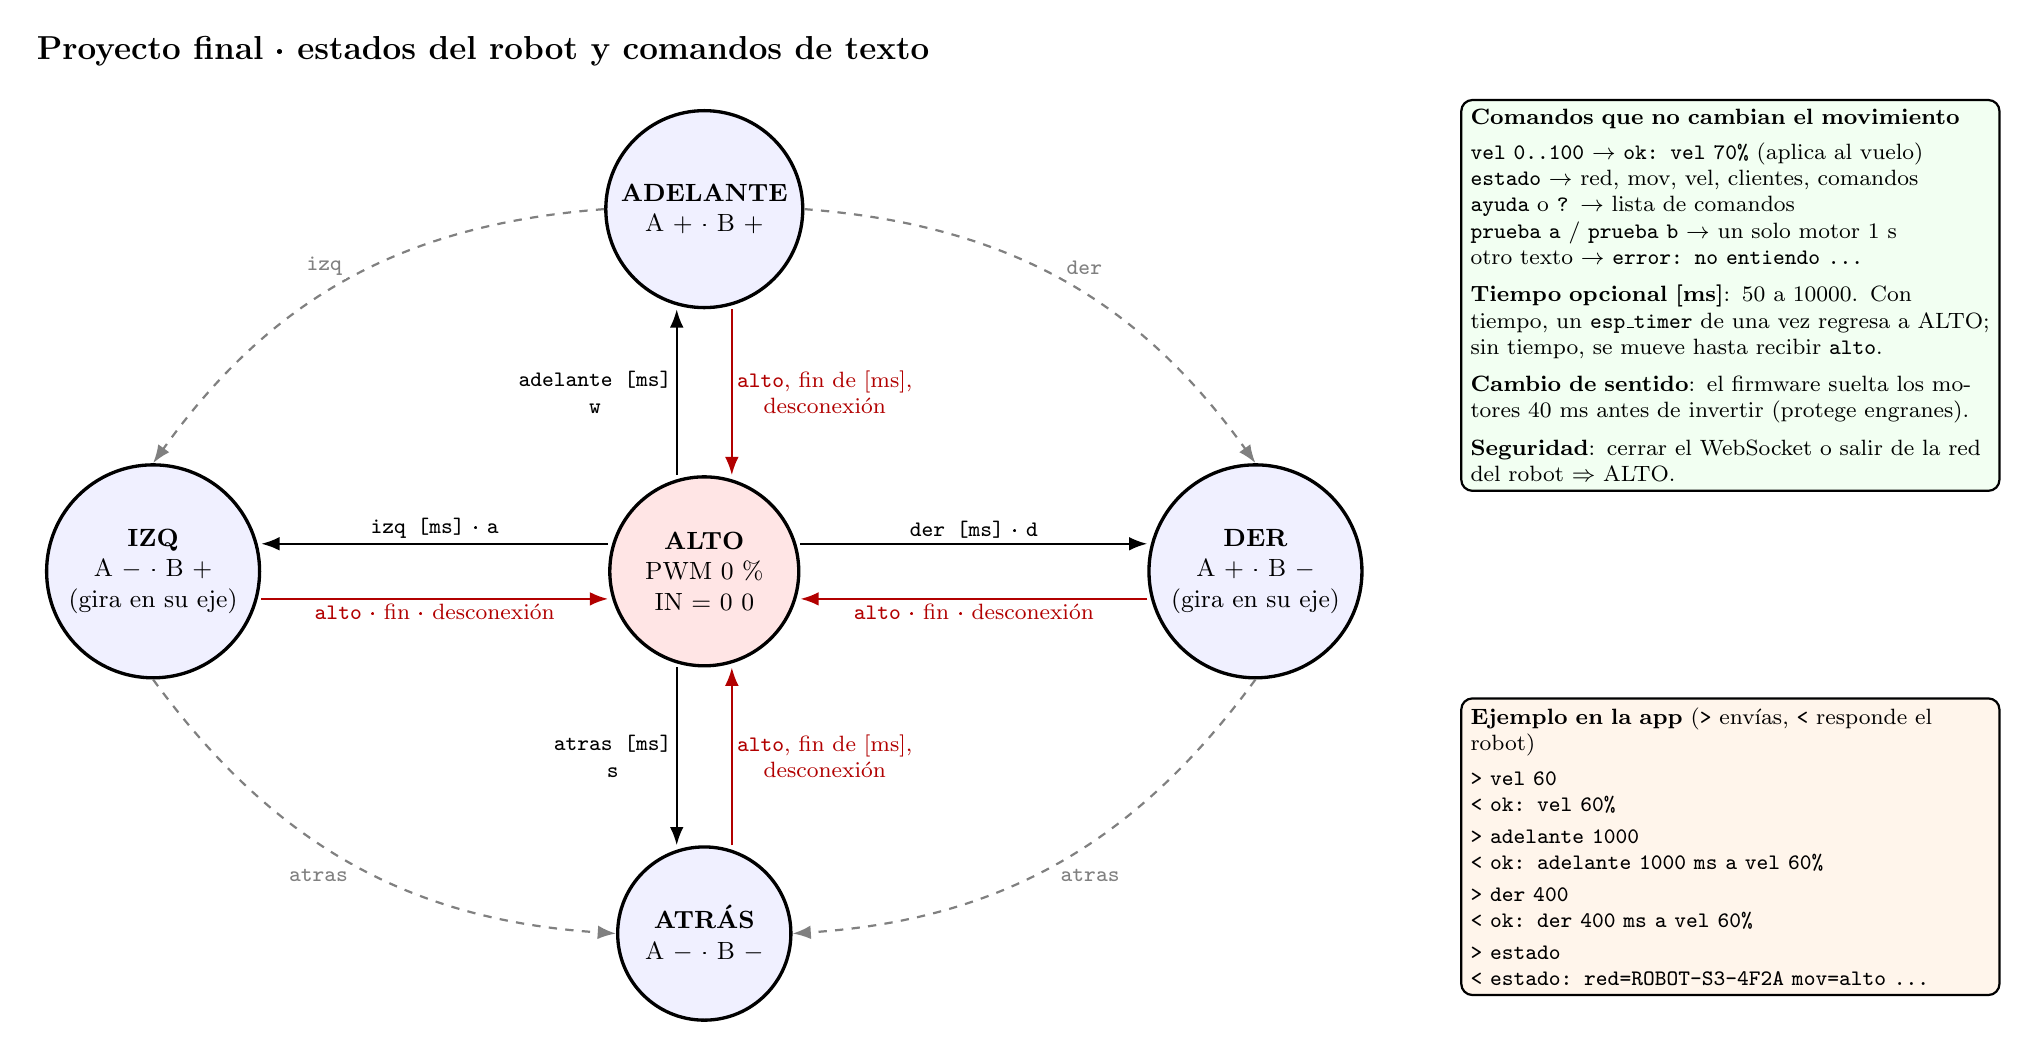
\begin{tikzpicture}[>=Latex,font=\small,
 st/.style={draw,very thick,circle,minimum size=2.2cm,align=center,fill=blue!6},
 al/.style={draw,very thick,circle,minimum size=2.4cm,align=center,fill=red!10},
 lab/.style={font=\footnotesize,fill=white,inner sep=1.5pt,align=center}]
\node[font=\large\bfseries,anchor=west] at (-8.6,6.6) {Proyecto final · estados del robot y comandos de texto};

\node[al] (alto) at (0,0) {\textbf{ALTO}\\PWM 0 \%\\IN = 0 0};
\node[st] (ad) at (0,4.6) {\textbf{ADELANTE}\\A $+$ · B $+$};
\node[st] (at) at (0,-4.6) {\textbf{ATRÁS}\\A $-$ · B $-$};
\node[st] (iz) at (-7.0,0) {\textbf{IZQ}\\A $-$ · B $+$\\(gira en su eje)};
\node[st] (de) at (7.0,0) {\textbf{DER}\\A $+$ · B $-$\\(gira en su eje)};

\draw[->,thick] ($(alto.north)+(-0.35,0)$) -- node[lab,left]{\texttt{adelante [ms]}\\\texttt{w}} ($(ad.south)+(-0.35,0)$);
\draw[->,thick,red!70!black] ($(ad.south)+(0.35,0)$) -- node[lab,right]{\texttt{alto}, fin de [ms],\\desconexión} ($(alto.north)+(0.35,0)$);
\draw[->,thick] ($(alto.south)+(-0.35,0)$) -- node[lab,left]{\texttt{atras [ms]}\\\texttt{s}} ($(at.north)+(-0.35,0)$);
\draw[->,thick,red!70!black] ($(at.north)+(0.35,0)$) -- node[lab,right]{\texttt{alto}, fin de [ms],\\desconexión} ($(alto.south)+(0.35,0)$);
\draw[->,thick] ($(alto.west)+(0,0.35)$) -- node[lab,above]{\texttt{izq [ms]} · \texttt{a}} ($(iz.east)+(0,0.35)$);
\draw[->,thick,red!70!black] ($(iz.east)+(0,-0.35)$) -- node[lab,below]{\texttt{alto} · fin · desconexión} ($(alto.west)+(0,-0.35)$);
\draw[->,thick] ($(alto.east)+(0,0.35)$) -- node[lab,above]{\texttt{der [ms]} · \texttt{d}} ($(de.west)+(0,0.35)$);
\draw[->,thick,red!70!black] ($(de.west)+(0,-0.35)$) -- node[lab,below]{\texttt{alto} · fin · desconexión} ($(alto.east)+(0,-0.35)$);
% cambios directos entre movimientos
\draw[->,thick,dashed,gray] (ad.west) to[bend right=25] node[lab,above left]{\texttt{izq}} (iz.north);
\draw[->,thick,dashed,gray] (ad.east) to[bend left=25] node[lab,above right]{\texttt{der}} (de.north);
\draw[->,thick,dashed,gray] (iz.south) to[bend right=25] node[lab,below left]{\texttt{atras}} (at.west);
\draw[->,thick,dashed,gray] (de.south) to[bend left=25] node[lab,below right]{\texttt{atras}} (at.east);

% Cuadro de comandos que no cambian de estado
\node[draw,thick,rounded corners,fill=green!5,anchor=north west,text width=6.6cm,align=left,font=\footnotesize] at (9.6,6.0) {%
\textbf{Comandos que no cambian el movimiento}\\[3pt]
\texttt{vel 0..100} $\to$ \texttt{ok: vel 70\%} (aplica al vuelo)\\
\texttt{estado} $\to$ red, mov, vel, clientes, comandos\\
\texttt{ayuda} o \texttt{?} $\to$ lista de comandos\\
\texttt{prueba a} / \texttt{prueba b} $\to$ un solo motor 1 s\\
otro texto $\to$ \texttt{error: no entiendo ...}\\[4pt]
\textbf{Tiempo opcional [ms]}: 50 a 10000. Con tiempo, un \texttt{esp\_timer} de una vez regresa a ALTO; sin tiempo, se mueve hasta recibir \texttt{alto}.\\[4pt]
\textbf{Cambio de sentido}: el firmware suelta los motores 40 ms antes de invertir (protege engranes).\\[4pt]
\textbf{Seguridad}: cerrar el WebSocket o salir de la red del robot $\Rightarrow$ ALTO.};
\node[draw,thick,rounded corners,fill=orange!8,anchor=north west,text width=6.6cm,align=left,font=\footnotesize] at (9.6,-1.6) {%
\textbf{Ejemplo en la app} (\texttt{>} envías, \texttt{<} responde el robot)\\[3pt]
\texttt{> vel 60}\\ \texttt{< ok: vel 60\%}\\[2pt]
\texttt{> adelante 1000}\\ \texttt{< ok: adelante 1000 ms a vel 60\%}\\[2pt]
\texttt{> der 400}\\ \texttt{< ok: der 400 ms a vel 60\%}\\[2pt]
\texttt{> estado}\\ \texttt{< estado: red=ROBOT-S3-4F2A mov=alto ...}};
\end{tikzpicture}
\end{document}
